\chapter{Toolchain Backend}\label{chap:offline_tezos}
After parsing and transforming a list of assertions, the resulting ASTs are passed to the target-specific backend. For this thesis, the platform target is Tezos, with Michelson as the compilation target. The pipeline stages of the backend comprise the ones colourized in \figref{fig:pipeline_backend}. First, the generic ASTs are subjected to a semantic check, which rejects any assertions containing unsupported types, operations or other invalid expressions. Valid ASTs are then cast to a target specific AST type and passed to the type checker. In this stage, the assertions are linked to the respective parent entrypoints, based on the parameter patterns and tags. Given the list of target specific ASTs and a linking, the compiler finally generates target code. Each stage is described in more detail in \secref{sec:backend_impl}.

As a preliminary and preparation for the compiler implementation, \secref{sec:ext_michelson} identifies necessary extensions to Michelson and Tezos' VM, in order to facilitate the distributed assertion scheme. Although the extensions are formalized in this thesis, implementing the extension is part of the protocol amendment. Furthermore, the compiler needs to generate the target code according to an on-chain orchestration scheme between the assertion and parent contract. This orchestration includes the mechanism to trigger several assertion checks per validator based on \eqref{eq:test_runs}, which was derived in the previous chapter. \secref{sec:orchestration} explores possible strategies for such a scheme, and discusses their strengths and weaknesses. Based on a resulting proposal for the orchestration, \secref{sec:cost_analysis_distributed} performs a cost analysis of distributed assertion checking and evaluates if, and under which conditions, it can increase the scalability in blockchain applications.

As a foundation for the other sections, \secref{sec:tezos} provides important background on the Tezos blockchain, its built-in smart contract language Michelson and some relevant tools and projects within its ecosystem.

\section{Introduction to Tezos}\label{sec:tezos}
The Tezos blockchain is presented in its whitepaper as a \enquote{generic and self-amending crypto-ledger} \cite{goodman_tezos_2014}. It uses a proof-of-stake consensus mechanism, which is not only used to agree on the current state of its ledger, but also allows its stakeholders to come to a consensus about changes in the economic protocol by participating in a voting process. The changes included in a protocol upgrade, called amendment, can influence, i.a., which transactions are valid on the blockchain, the payment system or even the voting process itself. It does so without risking a fork of the blockchain. Everyone owning the cryptocurrency of Tezos, called Tez, is considered a stakeholder and can participate in the consensus mechanism. The whitepaper compares the self-amending protocol of Tezos to a game created by Philosopher Peter Suber called ``Nomic'', whose set of rules are subjected to a democratic voting system \cite{nomic}. Similar concepts can also be found in modern pop culture, such as the virtual sports league ``Blaseball'' \cite{blaseball}, which became popular during the COVID-19 pandemic.

In addition to user accounts associated with a public key, Tezos supports smart contracts, which are written in the built-in language Michelson. Tezos' transaction fee system is similar to Ethereum's \cite{wood_ethereum_2021} - it is gas-instrumented and besides a base fee, every operation and byte of storage during contract execution has to be paid for by the user. However, Tezos imposes a hard cap on the amount of gas that can be consumed per operation (including internal transactions) \cite{tezos_docs}\cite{morley_gasmodel}, whereas Ethereum limits the gas quota only in respect to blocks \cite{wood_ethereum_2021}.\\
Tezos is written in the multi-paradigm programming language OCaml. Compiling its source code yields five essential binaries: the  node, baker, endorser, accuser and client. The node is the entity connecting to the peer-to-peer network and keeping a copy of the chain. Bakers are responsible for producing new blocks, the endorsers for validating new blocks and the accusers to call out bakers or endorsers which double-sign or -endorse. The client provides a command line interface to interact with nodes through remote procedure calls (RPC). 

\subsection{Proof-of-stake in Tezos}
In Tezos, contracts which have staked a minimum amount of tokens (called a roll), can participate in the consensus mechanism. When participating, a contract has a chance to obtain the role of either a baker or an endorser. Contracts not owning enough tokens or infrastructure to participate directly, can delegate their baking and endorsing rights to other contracts. The rights to bake or endorse are determined and assigned at the beginning of each cycle, which consists of a specified number of blocks. For baking, a random roll is selected for each block level and the rights are assigned to its owner. The block produced by that baker is signed by a fixed number of endorsers\footnote{For consistency, endorsers are referred to as ``validators'' in the remainder of this chapter} (32 as of protocol 007 Delphi), which also have been assigned endorsing rights for this block level by a random selection of rolls. Since participants can stake more than one roll, they may be assigned several endorsement slots at the same block level.

As an incentive for active participation in the consensus algorithm, delegates (and also delegators) receive rewards in form of tokens. However, if accusers detect double-baking or -endorsement, the delegate is penalized by burning (i.e., destroying) their security deposit.

\subsection{Michelson}
Michelson is a lower-level, stack-based language with strict type-checking. It supports primitive data types, like integers or strings, as well as high-level data structures, such as list, maps and sum types. The type system reduces the occurrence of runtime errors and ensures that only well-typed contracts are originated on the blockchain.

The concrete syntax of Michelson is called Micheline. A program is represented as Micheline nodes, which can be one of the following constructs:
\begin{itemize}
\item A constant of type integer (in decimal notation)
\item A constant of type string
\item A byte sequence in hexadecimal notation
\item An application of a language primitive to a sequence of nodes
\item A sequence of nodes
\end{itemize}
For documentation, readability and additional type constraints, Michelson and Micheline also offer three types of annotations - type, variable and field or constructor annotations, which are labelled with a unique special character in Micheline. The toplevel structure of a smart contract consists of a sequence of the three primitives \texttt{parameter, storage} and \texttt{code}. They declare the type of the input parameter, the storage type and the script, which is interpreted when the contract is invoked. The full grammar of Micheline and Michelson can be found in the Tezos developer resources \cite{tezos_docs}.

\subsubsection{Entrypoints}
Unlike Ethereum's contract language Solidity, Michelson doesn't have a concept of named functions with a dedicated parameter type. Instead of named functions, Michelson contracts model separate entrypoints by taking a sum type as an input parameter. The type constructors can optionally be tagged with a field annotation, which can be considered  as an entrypoint name. The sum type is built by nesting the \texttt{or} data type, which has the constructors \texttt{left} and \texttt{right}. As an example, the contract in \lstref{lst:entrypoints} has two entrypoints --- entrypoint \texttt{A}, which expects an integer wrapped in the \texttt{left} constructor, e.g. \texttt{left 1}, and entrypoint \texttt{B}, which expects a string wrapped in the \texttt{right} constructor, e.g. \texttt{right "hello world"}.
\begin{lstlisting}[language=Michelson, numbers=none, caption=Michelson contract with two entrypoints, label=lst:entrypoints]
parameter (or (int %A) (string %B));
storage unit;
code {
  ...
  IF_LEFT { ... (* entrypoint A *)}
          { ... (* entrypoint B *)}
}
\end{lstlisting}
By adding the constructor annotations \texttt{A} and \texttt{B}, the entrypoints can be invoked explicitly. The passed parameter value is then wrapped automatically into the respective constructor. Furthermore, it is possible to declare a \texttt{default} entrypoint, which is invoked when no explicit tag is specified in the transaction. By default, the default entrypoint is assigned to the root of the parameter type.

\subsubsection{Internal Operations}\label{sec:internal_ops}
Smart contracts are able to invoke other contracts by emitting internal operations. The return type of Michelson programs (more specifically, the type of the top element on the stack after the completed execution) is a tuple of a list of internal operations and the updated storage. After a contract completes, the operations in the returned list are run in sequence. Since internal operations may in turn also emit internal operations, the interpreter puts all emitted operations into a queue, which is processed in order. As an example, \figref{fig:internal_ops} shows an execution order of two external transactions and their internal operations in sequence.
\begin{figure}[h]
\centering
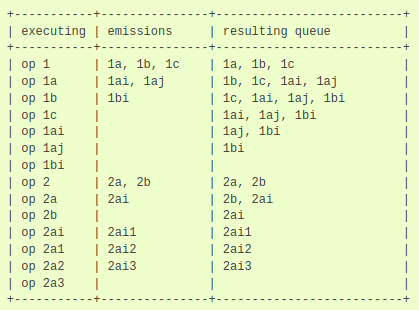
\includegraphics[width=0.5\linewidth]{figures/5-offline_tezos/internal_ops}
\captionsource{Execution order of two external operations and their internal operations}{\cite{tezos_docs}}
\label{fig:internal_ops}
\end{figure}

Both external and internal operations can fail, if the source contract does not have enough balance to spend the specified amount, a gas limit was reached, or if a program fails due to reaching a \texttt{FAILWITH} instruction. If a failure occurs, the whole sequence fails and all changes up to the point of failure are reverted. Within a sequence, an operation can thus have one of the following result types:
\begin{itemize}
\item \textbf{Applied} --- the operation was successful
\item \textbf{Failed} --- the operation failed
\item \textbf{Skipped} --- the operation was in sequence after a failed operation
\item \textbf{Backtracked} --- reverted operation due to a failed operation further along in the sequence
\end{itemize}

\subsection{Gas Model}
Tezos stores and transmits data as byte sequences --- in order to obtain a typed representation of their value for interpretation, a byte sequence is first deserialised into Micheline and subsequently parsed into a typed AST. Conversely, before transmitting or storing something on the blockchain, the typed representation is first unparsed into Micheline and then serialised. Since these working steps also entail computational effort, they consume gas and thus account for some of the transaction fees. The gas consumption of an operation (e.g., a transaction or a contract origination) is thus composed of the following positions on top of a base gas fee \cite{morley_gasmodel}\cite{tezos_repo}:
\begin{enumerate}
\item \textbf{Reading costs} --- apply for reading the contract code and storage from the blockchain and depend on the amount of bytes read
\item \textbf{Deserialization costs} --- depend on the components of the Micheline expression and the size of the byte sequence. Apply lazily, thus the deserialization of each value only has to be paid for once
\item \textbf{Parsing costs} --- are composed of three types of costs:
	\begin{itemize}
	\item type parsing --- apply when a Micheline node is converted into a valid type
	\item data parsing --- apply when a node is converted into the value of a known type and depends on the size of the value
	\item code parsing --- apply when the instructions of a program are type checked and depends on the number and types of instructions. Some instructions are expensive, such as \texttt{IF} (both branches need to be checked and compared) or \texttt{CREATE\_CONTRACT} (requires type check of the invoked contract)
	\end{itemize}
\item \textbf{Type comparison costs} --- apply when types are checked for equality (e.g. when type checking the branches of the \texttt{IF} instruction) or during contract interpretation
\item \textbf{Interpretation costs} --- apply for each interpreted instruction and depend on their computational complexity.
\item \textbf{Unparsing costs} --- apply when converting typed data to untyped Micheline nodes and depend on the data type and size
\item \textbf{Serialization costs} --- apply when serializing Micheline nodes to byte sequences and depend on the expression and its size
\item \textbf{Writing costs} --- apply when writing to the internal database and depend on the amount of bytes. A base gas fee is burned for each additional byte of storage.
\end{enumerate}
If a transaction emits internal operations, their gas consumption is computed in the same way and is added to the total gas consumption of the external operation.

\subsection{Developer Tools in the Tezos Ecosystem}
This section describes some tools and projects within Tezos' ecosystem, which are relevant to the development of the toolchain or the protocol amendment.

\subsubsection{Tezos Libraries}
Tezos' executables and libraries are available on OCaml's package manager \texttt{opam} \cite{tezos_opam}. The protocol libraries of every version are released separately, thus any projects can be built on the protocol of choice. Relevant libraries included in the backend of the toolchain are, i.a, the Micheline library containing the internal abstract syntax tree (AST) and parser of the Michelson language, the protocol libraries providing functions to type check code or data, and client libraries to retrieve any needed information from the node or blockchain via wrapped RPCs.

\subsubsection{Testing Tools}
Before a new protocol is proposed to the Tezos network, it has to be thoroughly tested with system, integration and regression tests. This requires a sandboxed network to simulate the real peer-to-peer network. Tezos' development environment provides the two testing frameworks Flextesa (Flexible network sandboxes)\cite{tezos_docs} and its successor Tezt \cite{tezos_docs}. They allow to configure and run a small, fully functional sandboxed test network including nodes, bakers, endorsers and accusers. Besides testing new protocols, they can also be used to interactively test smart contracts.

\subsubsection{High-level Languages}\label{sec:languages}
Michelson is a compilation target for various high-level languages that provide a more user-friendly and intuitive way of writing smart contracts. Additionally, some of them provide development environments, testing or verification tools. The following list introduces three prominent languages, which compile to Michelson:
\begin{description}
\item[\textbf{Liquidity}] \cite{liquidity} is a language with an OCaml-like syntax, which allows to express contracts in a functional way. It supports using local variables instead of stack manipulations. Its module system can be used to write reusable contract code or libraries. Besides an optimizing compiler, the project also includes a decompiler to compile Michelson programs to Liquidity source code.
\item[\textbf{SmartPy}] \cite{smartpy} is a language available through a Python library and lets developers write contracts and tests using Python syntax and structures (such as classes). Its developer suite includes, i.a., a compiler, a simulation engine for testing contracts and an online editor.
\item [\textbf{Ligo}] \cite{ligo} offers multiple syntax flavours close to Pascal, OCaml or Reason. Besides compilation, the toolchain allows to invoke or evaluate the generated code locally. The project provides Ligo as OCaml packages, which can be integrated into other projects.
\end{description}

\section{Extensions to Michelson}\label{sec:ext_michelson}
For the assertion code to be executable by the VM of Tezos, Michelson and the VM have to be extended with new instructions. This includes an instruction to generate a random value of some primitive data type non-deterministically. The formalization and possible implementation of such an instruction is described in \secref{sec:random}. Aside from this, many useful use-cases involve checking random elements of lists, and possibly strings or bytes. For convenience, it is worth considering adding indexing operations for some data types to the VM. This is discussed in more detail in \secref{sec:nth}.

As a foundation for the formalization of these new instructions, \secref{sec:michelson_semantics} gives a brief introduction to the Michelson interpreter and type system first.  

\subsection{Language Semantics and Type System}\label{sec:michelson_semantics}
Michelson is interpreted purely functional; the interpreter takes the current stack and an operation and builds a return stack from the initial one, without causing any side effects. The definition of the recursive interpreter is given in the form of a list of rules, comprising of all possible inputs (i.e., program and stack types) and the respective output stack type of the computation. Each rule is of the following form: 
\begin{lstlisting}[caption=Selection rules in the Michelson interpreter \cite{tezos_docs}, language=, numbers=none, label=lst:rules]
> (syntax pattern) / (initial stack pattern)  =>  (result stack pattern)
    iff (conditions)
    where (recursions)
    and (more recursions)
\end{lstlisting}
For each valid program and initial stack, exactly one rule applies. Following the keyword \texttt{iff}, the rule can add extra conditions over values on the stack. If the result depends on the results of other program interpretations, such as conditionals or function calls, the rule can contain recursive rules in the \texttt{where} or \texttt{and} clauses. These clauses represent a recursive interpretation of an intermediate program. The rule thus only applies, if the interpretation of the intermediate result matches the expected pattern.

The type system of Michelson consists of typing rules for each syntax construct, restricting the valid input stacks. The typing rules use the meta variables \texttt{'a} for type, and \texttt{'A} for stack type variables. Using these meta variables, the rules express consistency within the program. The typing rules are given in the form shown in \lstref{lst:type_rules}, where premises are additional typing requirements over values on the stack:
\begin{lstlisting}[caption=Form of typing rules in Michelson's specification \cite{tezos_docs}, language=, numbers=none, label=lst:type_rules]
(syntax pattern)
:: (type of stack before) -> (type of stack after) [rule-name]
   iff (premises)
\end{lstlisting}
The Tezos developer resources \cite{tezos_docs} provide a comprehensive list of type notations, syntax and stack patterns.

Since the Michelson language and interpreter are implemented in the protocol-specific libraries of Tezos, adding new instructions require a protocol update. This entails adding the new instruction to the list of tokens, adding one or several selection rules to the interpreter and typing rules to the type checker \cite{tezos_repo}. Furthermore, the protocol must specify the gas cost of its computation. Previous extensions to the Michelson language, such as the addition of the instruction ``\texttt{DIG n}'' in protocol 005 Babylon \cite{tezos_michelson_ext}, can be used as a guideline for the extension. The gas cost specification of existing instructions should be used as an orientation in specifying the costs of new instructions.

\subsection{Random Instruction}\label{sec:random}
Since smart contracts generally need to be deterministic, s.t. the network can reach a consensus about the state of the ledger \cite{chatterjee_probabilistic_2019}, the prevalent workarounds for generating pseudo-random numbers cannot be used to implement the random generators in assertion contracts. The scheme explicitly requires the validators to check distinct elements in the search space. Common schemes for obtaining random values, like oracles or using block attributes as seeds \cite{chatterjee_probabilistic_2019}, would generate the same values for all validators. Thus, the VM needs to provide an instruction to generate a ``real'' random value exclusively for assertion checking. In order to preserve the deterministic behaviour of normal smart contracts, the instruction should not be available in the normal execution mode.

\lstref{lst:rand_type} specifies the typing and selection rule of a new instruction \texttt{random} for integers, although such an instruction could also be provided for other data types, such as \texttt{nat}, \texttt{string} or \texttt{mutez}. The selection rule for this instruction applies for the instruction identifier \texttt{RANDOM} and an input stack containing at least two elements. It consumes an offset and a positive range from the stack and pushes a randomly generated integer to the top. The typing rule (line 1) specifies, that the offset should be of type \texttt{integer}, and the range of type \texttt{nat} (i.e., a natural number).
\lstset{upquote=true}
\begin{lstlisting}[caption=Typing and selection rules of the integer \texttt{random} instruction, language=, showlines=true, label=lst:rand_type]
:: int : nat: 'A -> int : 'A
> RANDOM / offset : range : S  => int : S
\end{lstlisting}

Within the Michelson interpreter, the selection of rules is implemented as a huge match case \cite{tezos_repo}. If the rule for \texttt{random} applies, the instruction could be computed in OCaml as indicated in \lstref{lst:rand_impl}.
\begin{lstlisting}[caption=Simplified evaluation of \texttt{random} in the Michelson interpreter, language=, label=lst:rand_impl, float]
match (instruction, stack) with
...
| (Random (offset, (range, rest))) ->
   Random.self_init;
   let rand_int = offset + Random.int(range) in
   return (rand_int, rest)  (* resulting stack *)
\end{lstlisting}

\subsection{List Indexing}\label{sec:nth}
Michelson currently does not provide any predefined indexed access operators for data types like lists, strings or bytes. Accessing a random element of a sequence can, of course, be implemented using low-level instructions. However, because such operations are used frequently in many of the given use-cases, adding it as a predefined primitive for some data types might be justifiable. It reduces the required code to express the indexing, and thus not only improves the readability of the contract code, but also lowers the costs of the contract origination and execution.

\lstref{lst:nth_type} specifies the typing and selection rules of an instruction \texttt{nth} to access the element of a list at a specified index. It consumes a list with elements of type \texttt{'a}, and an index of type \texttt{nat} from the top of the stack. After the computation, on top of the resulting stack is an optional value of the element type \texttt{'a}. A selection rule (line 2 and 3) is given for each of the two possible result stack patterns, i.e., a value of type \texttt{'a} or an undefined value if the given index is out of bounds.
\begin{lstlisting}[caption=Selection and type rule of the list \texttt{nth} instruction, language=, label=lst:nth_type]
:: (list 'a) : nat : 'A -> option 'a : 'A
> NTH / l : index : S  =>  Some 'a: S
     iff index is within bounds
> NTH / l : index : S  =>  None 'a: S
     iff index is out of bounds
\end{lstlisting}

Within the VM, Michelson lists are represented with OCaml's list type --- the computation of \texttt{nth} thus simply calls the \texttt{nth} function of OCaml's List module, as indicated in \lstref{lst:nth_impl}. \\
\begin{lstlisting}[caption=Simplified evaluation of \texttt{nth} in the Michelson interpreter, language=, label=lst:nth_impl]
match (instruction, stack) with
...
| (Nth ({elements = []; _}, (_, rest))) ->
  return ((None, rest)
| (Nth ({elements = es; length}, (index, rest))) ->
  let l_length = of_int length in
  if index <= l_length
    then return (Some (List.nth es index), rest)
    else return (None, rest)
\end{lstlisting}
\lstset{upquote=false}

As stated above, the indexing operation can also be translated to a sequence of already existing instructions. Michelson features instructions to execute a loop or iterate over a list, which can be used for such an implementation. An exemplary and readable implementation of the operation \texttt{nth} for lists in the high-level language Liquidity is given by \lstref{lst:nth_liq} in appendix \ref{apx:nth}\footnote{Since Michelson is a low-level language, code examples in this chapter are mostly provided in Liquidity to provide a short and readable representation of the contract structure or logic. In most cases, the corresponding Michelson code generated by the Liquidity compiler is included in the appendix.}. The appendix also contains the corresponding Michelson code after compiling the source with the Liquidity compiler (\lstref{lst:nth_tz}).

\section{Orchestration of Contract and Assertions}\label{sec:orchestration}
So far, the assertion and parent contract have been considered separately. However, they have to be orchestrated on the blockchain, such that the assertion code is either invoked automatically before the parent code is executed, or the assertion code can be selectively invoked by the validators. Furthermore, the orchestration should include a mechanism to determine and trigger the required number of test runs per validator. Depending on the orchestration strategy, the compiler then assembles and translates the assertion and parent code into one or several smart contracts.

This section describes two possible approaches for an orchestration --- a monolithic and a modular approach. It also discusses, which of the given architecture is chosen for the proof-of-concept implementation, and why.

\subsection{Monolithic Orchestration}\label{sec:monolithic}
In the monolithic approach, the assertion and parent code are merged into a single smart contract. This tightly couples and unites the code in one self-contained unit. As shown in \figref{fig:mono_eps}, the assertions are appended to the original contract as separate entrypoints. Since the \texttt{random} instruction is only available in the execution mode for assertion checking, the assertion code cannot be directly prepended to the respective production code. Otherwise, transactions invoking such an entrypoint could not be included into blocks, as these are validated in the normal execution mode.
\begin{figure}[h]
\centering
  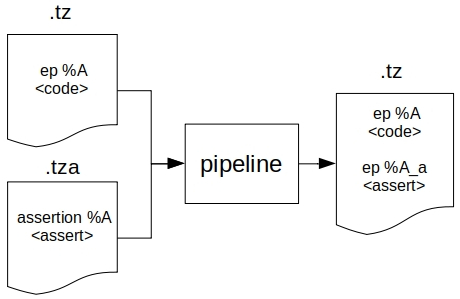
\includegraphics[width=0.5\textwidth]{figures/5-offline_tezos/pipeline_output_mono_ep_basic.jpg}
	\caption{Monolithic assembly - appending assertions as separate entrypoints}
	\label{fig:mono_eps}
\end{figure}

The interface of the contract should make apparent, which of the entrypoints contain production, and which contain their respective assertion code. This can be solved by using fixed tag patterns for assertion entrypoints, which can be derived from the parent entrypoint tag. \figref{fig:mono_eps} proposes the tag suffix ``\texttt{\_a}'' for assertion entrypoints. External transactions should only invoke the production entrypoints.

The assembly in \figref{fig:mono_eps}, however, does not yet provide any means to trigger several test runs per validator. Since the required number of test runs $t$ can only be determined at runtime, it cannot be passed to the validators as a parameter to the validation request. Instead, the contract itself should contain a controller to handle the calculation of $t$ and the initiation of $t$ test runs. Similar to the assertion code, such a controller can be appended as another separate entrypoint, as shown in \figref{fig:monolithic_orchestration}. Instead of invoking the assertion entrypoint (\texttt{A\_a}), the validators would then invoke the controller entrypoint (\texttt{A\_c}), which determines $t$ and invokes (\texttt{A\_a}) $t$ times as an internal operation.
\begin{figure}[h]
\centering
  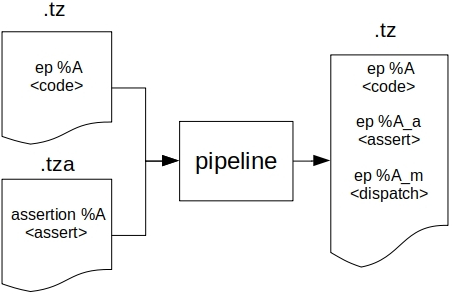
\includegraphics[width=0.5\textwidth]{figures/5-offline_tezos/pipeline_output_mono_ep}
	\caption{Monolithic assembly with separate entrypoints for controller and assertion}
	\label{fig:monolithic_orchestration}
\end{figure}

As a hybrid solution between a monolithic and a modular approach, the controller can be implemented as a separate smart contract, which operates as a proxy. This contract is invoked in place of the monolithic contract, which in turn invokes the original or assertion entrypoints as internal operations. The implementation of the modular part can be adopted from \secref{sec:modular}.

If a developer does not specify an assertion for all entrypoints of the parent contract, invoking their non-existing controller entrypoints would cause a transaction failure. In order to avoid this and increase the robustness, the compiler should generate dummy controllers for empty assertions, which simply return unit (i.e, an empty list of internal operations and the unchanged storage).

\lstref{lst:mono_liq} implements a monolithic contract in Liquidity. The contract contains the two parent entrypoints \texttt{A} (line 3) and \texttt{B} (line 21), and provides an assertion entrypoint \texttt{A\_a} (line 5) for \texttt{A}. Entrypoint \texttt{B} does not have an associated assertion. For both parent entrypoints, it provides the controller entrypoints \texttt{A\_c} (line 7) and \texttt{B\_c} (line 23). Controller \texttt{A\_c} determines the number of test runs in line 8 (the implementation of the formula is omitted here) and creates $t$ internal operations, which invoke the assertion entrypoint with the same parameter (lines 9-17). These are then run in sequence afterwards. Controller \texttt{B\_c}, on the other hand, does not emit any operations and immediately returns. This code can never fail and thus accepts any input value for the parameter.
\lstinputlisting[label=lst:mono_liq, caption=Implementation of a monolithic contract in Liquidity, numbers=left]{listings/monolithic.liq}

\figref{fig:interaction_monolithic} depicts the resulting interactions of the nodes, validators and monolithic smart contracts on the blockchain. The execution model requires a dedicated mode for distributed assertion checking. A possible mechanism to activate this mode is using a special transaction type, which is denoted by \texttt{txa(destination, entrypoint, parameter)} in the graphic. When an operation, such as a transaction or origination, is injected into a node, it is normally propagated to the network after it has been pre-validated by the node. After the injection of \texttt{txa(1, \%A, parameter)}, however, the node broadcasts its derivation \texttt{txa(1, \%A\_c, parameter)} to the network, which invokes the controller entrypoint instead. If this operation finishes successfully for all validators, i.e., no counterexample is published on the network after a certain amount of block cycles, the node can finally broadcast the initial operation as a normal transaction. In case of an assertion failure, the respective validator broadcasts the counterexample including the generated random values. As a consequence of the broadcasted counterexample, the initial operation \texttt{txa(1, \%A, parameter)} should be reverted and rejected by the injecting node. How a counterexample is represented and included on the chain is an unresolved question --- \secref{sec:counterexample} picks this topic up and gives some ideas regarding possible implementations. 

\begin{figure}
\centering
  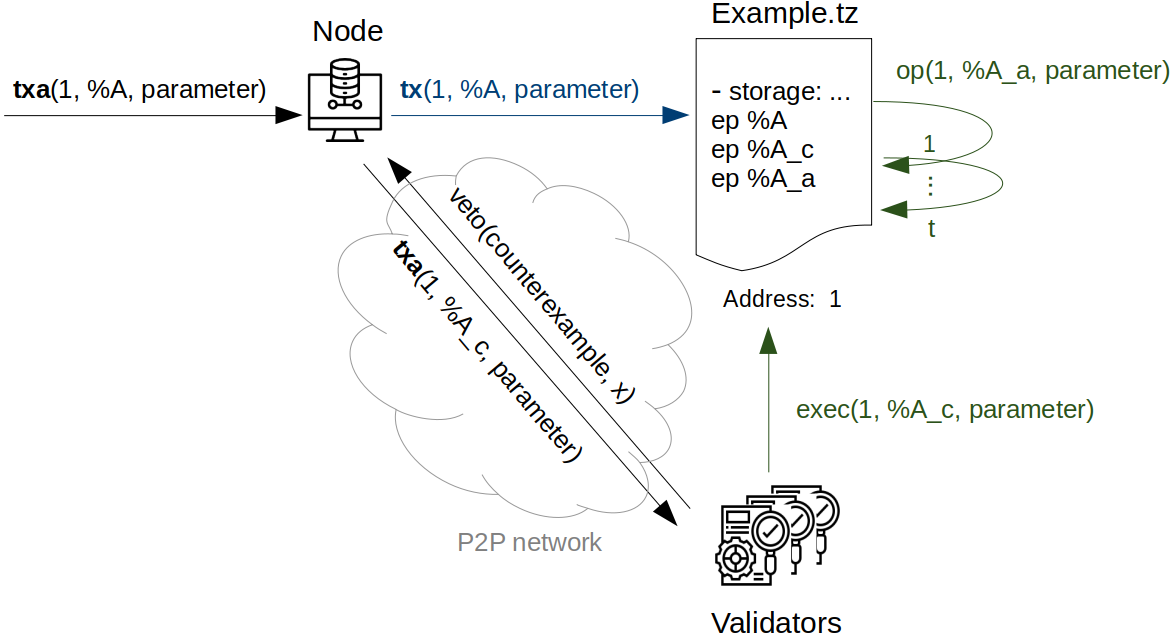
\includegraphics[width=0.9\textwidth]{figures/5-offline_tezos/interaction_monolithic_2}
	\caption{Interaction with a monolithic contract}
	\label{fig:interaction_monolithic}
\end{figure}

This orchestration scheme only works as described when using explicit entrypoint tags for the contract invocations. On the one hand, calling entrypoints implicitly (by wrapping the parameter in the respective sum type constructors) causes a type mismatch for the controller and assertion entrypoints. \lstref{lst:mono} shows the parameter type of the Michelson implementation corresponding to the contract given in \lstref{lst:mono_liq} --- entrypoint \texttt{A} can be invoked implicitly with parameter value \texttt{Left 4}. The respective assertion entrypoint \texttt{A\_a} expects the value as \texttt{Right (Right (Left 4))} and the controller \texttt{A\_c} as \texttt{Right (Right (Right (Left 4)))}. Calling these entrypoints with the same parameter is thus not possible. On the other hand, the explicit tags encode the link between production, controller and assertion code --- omitting them would dissolve all references between them. Hence, implicit entrypoint invocation cannot be supported in the execution mode of assertions. The assertion compiler thus needs to enforce the use of explicit entrypoints in the parameter type declarations and the \texttt{txa} operation type must expect a mandatory entrypoint specification as an argument.
\lstinputlisting[label=lst:mono, language=Michelson, caption=Skeleton of a monolithic contract in Michelson, numbers=left, float]{listings/monolithic.tz}

This thesis does not go into more detail about how the described execution model for a monolithic orchestration is designed and implemented in the blockchain protocol. What needs to be considered in future work concerning the protocol design is the separate execution mode, a dedicated operation type as proposed above, the derivation of a transaction which attempts to find a counterexample, the handling of assertion failures and the exclusive acceptance of the off-chain computation (and thus the transaction submitting it) or the counterexample.

\subsubsection{Evaluation of the Monolithic Approach}
The purely and hybrid monolithic implementation each have strengths and weaknesses. Generally, they share a pivotal disadvantage - they require a modification of the parent contract. This complicates the compilation process substantially and precludes the integration of assertions to contracts which have already been deployed to the blockchain. \lstref{lst:mono} shows how the parameter type and branching within the code body have to be adapted compared to the original parent contract in \lstref{lst:mono_parent}. Since the monolithic assembly results in deeper parameter and code nestings, the overall complexity of the contract increases and may obscure the production code.
\lstinputlisting[label=lst:mono_parent, language=Michelson, caption=Skeleton of the pure parent contract in Michelson, numbers=left]{listings/monolithic_parent.tz}

Another shortcoming is the missing support of implicit entrypoint invocations. Even though the previously mentioned measures can prevent transactions failures, this still poses a restriction in the interaction with smart contracts. 

Due to the tight coupling of parent and assertion code, this approach is also inflexible. Adaptions to either the assertion or the parent contract require a complete recompilation and origination of the monolithic contract. The hybrid solution resolves some of the tight coupling, as a new version of the controller contract can be originated independently of the monolithic contract.

Besides these disadvantages, the monolithic approach provides a distinct advantage: the production and controller entrypoints can be invoked independently, implicating that the validators do not have to run the production code while checking the assertion. Conversely, the assertion code is not rerun if the parameter was validated and the actual transaction is broadcast to the network. This reduces the transaction cost for the user, as well as the overall computational footprint of the transaction and the validation in the network.

\subsection{Modular Orchestration}\label{sec:modular}
In the modular approach, the controller and each of the assertions are originated as separate contracts on the blockchain. The controller mirrors the interface of the parent contract, while each assertion contract only features a single entrypoint, which corresponds to the raw type of the associated parent entrypoint. By keeping the assertion code separated, the parent contract remains pure and does not have to be modified. Similar to the hybrid solution mentioned in the monolithic approach, the controller calls the respective assertion contract $t$ times as an internal operation, before invoking the parent contract as operation $t+1$. In the case of empty assertions, the controller acts as a direct gateway by invoking the parent contract immediately. Corresponding to this architecture, the toolchain returns $m + 1$ contracts, where $m$ is the number of specified assertions in the input. The code assembly and output of the toolchain is outlined in \figref{fig:modular_assembly}.
\begin{figure}[h]
\centering
  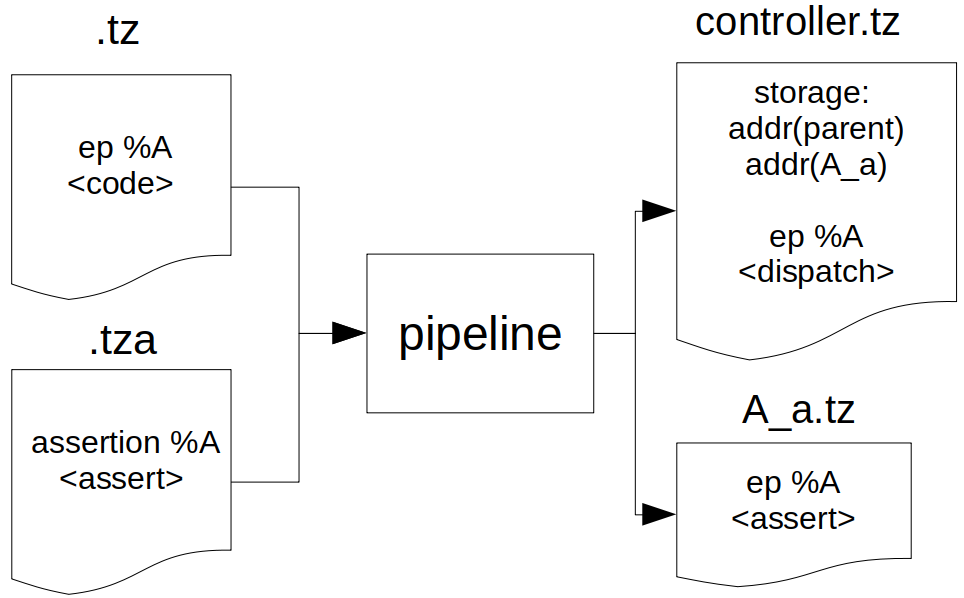
\includegraphics[width=0.6\textwidth]{figures/5-offline_tezos/pipeline_output_modular.png}
	\caption{Modular assembly of assertion and manager code}
	\label{fig:modular_assembly}
\end{figure}

In order to link the separate contracts to each other, the controller needs to have a reference to the other contract modules. This results in a fixed origination order --- the assertion and parent contracts must be originated first, and their addresses are passed to the controller as initial storage values. A proposed structure of the storage is a map from a unique identifier to an address. The entrypoints of the controller can then look up the addresses of the parent and the respective assertion contract with an assigned identifier. The assignment of the identifiers is hard-wired during the compilation, as is demonstrated in the rudimentary and simplified Liquidity implementation of a controller contract in \lstref{lst:manager_modular}. The corresponding storage initiation for this contract is the map $\lbrace 0 \rightarrow \langle \text{address parent} \rangle; 1 \rightarrow \langle \text{address assertion} \rangle \rbrace$ . The hard-wired identifiers are used in lines 5 and 6 to retrieve the addresses from the storage.
\lstinputlisting[label=lst:manager_modular, caption=Implementation of the modular controller in simplified Liquidity, language=Michelson, numbers=left]{listings/controller_basic.liq}

The interaction with the modular contracts is shown in \figref{fig:interaction_modular}. Even though the transactions shown in the diagram state an explicit entrypoint tag, the scheme also supports implicit entrypoint invocations. Invocations of the assertion contract pass the parameter as a raw value. The general execution model is similar to the model for the monolithic approach, but requires a few modifications; because the controller mirrors the interface of the parent contract, the \texttt{txa} operation can be broadcast to the network directly --- a derivation to a distinct transaction, which calls the assertion selectively, is not necessary. If none of the validators publish a counterexample, the initial transaction is broadcasted to the network as a normal operation to be included in a block. This transaction will inevitably rerun the assertion code in the normal execution mode (as it invokes the controller). Hence, the \texttt{random} instruction should not cause an internal operation to fail in the normal execution mode of the VM. This could be solved by marking these internal operations with the operation result ``Skipped'' (cf. \secref{sec:internal_ops}), or by introducing a dedicated result type for this case. 
\begin{figure}[h]
\centering
  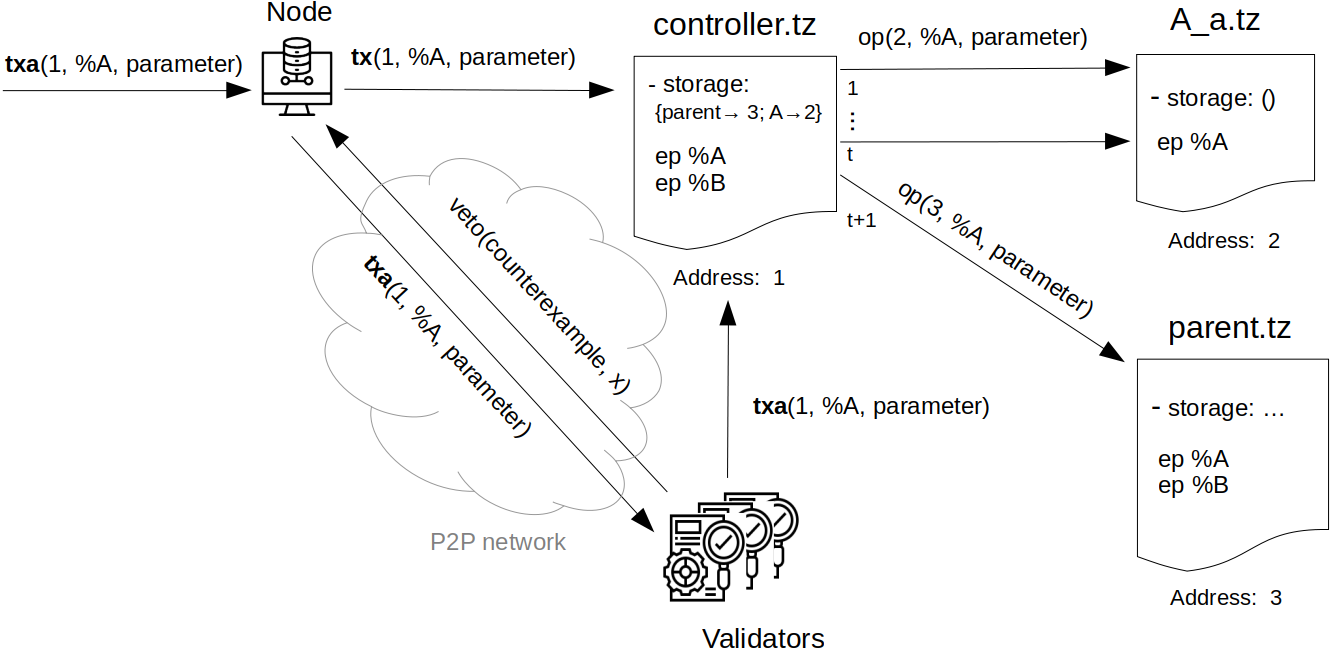
\includegraphics[width=\textwidth]{figures/5-offline_tezos/interaction_modular.png}
	\caption{Interaction with modular contracts}
	\label{fig:interaction_modular}
\end{figure}

\subsubsection{Evaluation of the Modular Approach}
This approach resolves the two crucial problems of the monolithic orchestration: by mirroring the interface of the parent contract, the parameters passed to the manager contract can be forwarded directly to the parent contract, regardless of whether the default or an explicit entrypoint was called. Furthermore, the parent contract does not need to be modified, which leads to a much simpler compilation process and allows to extend already originated contracts with assertions. Due to its modularity, adaptions to either contract do not necessarily require a recompilation and origination of all components, as the controller is the only component with tight coupling. In order to reduce this coupling, one could be inclined to add a setter entrypoint to the controller (as a sort of dependency injection). This, however, would break the mirroring of the parent contract and is thus not possible without annulling one of the key strengths of the design.

The approach essentially exhibits two weaknesses: firstly, the assertion and the parent cannot be called separately. As a result, the production code is run by every validator while searching for counterexamples. Moreover, the assertion code is also run when validating a block containing the accepted transaction. This increases the transaction cost for the user and requires a higher computational effort by the whole network. Secondly, it exposes a security vulnerability, given that assertions can be bypassed by calling the parent contract directly. This iteration of the design does not demand to close this vulnerability, hence possible solutions are not discussed in this thesis.

Even though the monolithic approach is expected to be more efficient, the toolchain implementation described in the following sections is based on the modular architecture. It is simple to implement, requires less modifications to the blockchain protocol and provides more flexibility.

\section{Backend Implementation}\label{sec:backend_impl}
The following sections describe the tasks and implementation of the pipeline stages in the toolchain backend.
\begin{figure}[h]
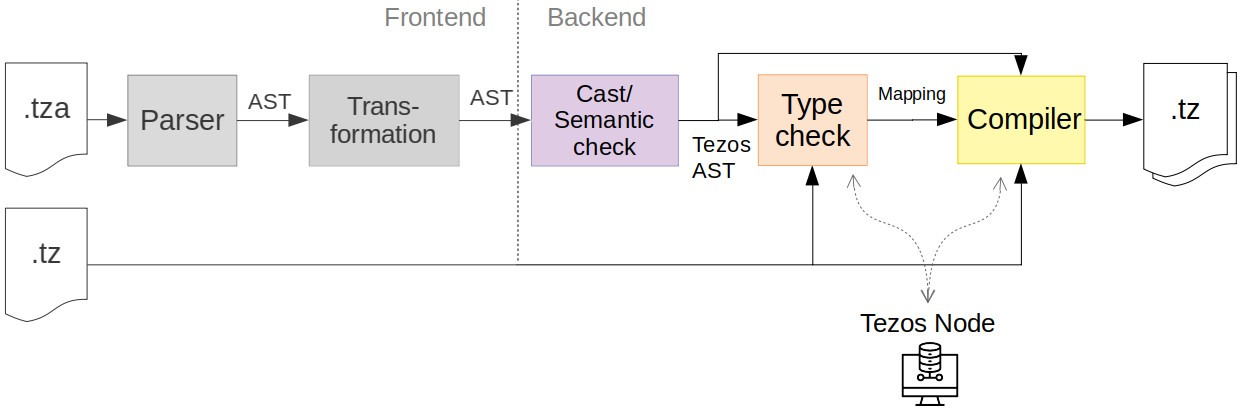
\includegraphics[width=\linewidth]{figures/5-offline_tezos/pipeline_backend}
\caption{The stages of Tezos-specific backend of the compilation pipeline}
\label{fig:pipeline_backend}
\end{figure}

\subsection{Interaction with Tezos Nodes}
Some stages of the backend have to interact with a Tezos node, e.g. to retrieve information from the blockchain. For this, the backend uses the Tezos client libraries, which provide high-level functions wrapping RPCs to a configured node. The command-line interface of the toolchain provides options for configuring the host address and port of the RPC interface to connect to a specific local or public node. By default, the toolchain tries to connect to a local node on the default port.

\subsection{Semantic Analysis}
After the transformation, the frontend passes a list of ASTs to the backend. Because the frontend was designed to be generic, they may contain type, operations or expressions which are not supported by the target language. Therefore, the semantic check should reject any input which cannot be translated to Michelson.

As an additional restriction, quantifiers should only bind variables of primitive data types. As the majority of use-cases seem to require quantification over numerical values, the current implementation of the semantic check restricts predicate variables to the types \texttt{int} and \texttt{nat}. Future iterations of the toolchain and protocol may add support for other primitive types, such as \texttt{string} or \texttt{bytes}.

Semantic rules imposed by Michelson do not have to be checked explicitly by the toolchain --- the RPC interface of Tezos nodes provides a function to parse and type check Michelson programs, which can be used to verify the correctness of the compilation result and reject any assertions containing type or other semantic errors.

If the semantic check was successful, the module returns the assertions as a list of Tezos-specific ASTs. \lstref{lst:tezos_ast_type} shows the toplevel definition of this AST type.
\begin{lstlisting}[label=lst:tezos_ast_type, language=, numbers=none, caption=Toplevel Tezos-specific AST type definition in OCaml]
type tezos_ast =
  {entrypoint : string * pattern; body : assertion}
\end{lstlisting}
As Tezos is currently the only supported target platform, the type differs only slightly from the generic type. If the assertion does not specify an explicit entrypoint tag, the optional value is replaced with Tezos' notation for the default entrypoint. The subtree types for the parameter pattern and the assertion remain equivalent to the generic subtree types.

\subsection{Type Check}\label{sec:typecheck}
Given a list of Tezos-specific ASTs, the task of the type checker is to link each AST to the respective entrypoint of the parent contract. This stage module can therefore also be referred to as the ''linker``. The linking is needed by the compiler to correctly assemble and type the controller and assertion contracts. As a simple example, the linker should correctly assign the AST of the first assertion in \texttt{Example.tza} (\lstref{lst:linker_assertion}) to entrypoint A and the second assertion to entrypoint B of the parent contract \texttt{Example.tz} (\lstref{lst:linker_parent}). 

\vspace{\baselineskip}
\noindent
\begin{minipage}{.45\textwidth}
\begin{lstlisting}[label=lst:linker_parent, numbers=none, language=Michelson, caption=Example.tz]
parameter (or (int %A)
              (string %B));
...
\end{lstlisting}
\end{minipage}\hfill
\begin{minipage}{.5\textwidth}
\begin{lstlisting}[label=lst:linker_assertion, numbers=none, language=Assertion, caption=Example.tza]
(entrypoint %A (i : int) ...)
(entrypoint %B (s : string) ...)
\end{lstlisting}
\end{minipage}
\vspace{\baselineskip}

Because explicit entrypoint tags are optional in Michelson contracts, the linking is primarily done by type matching between the declared parameter types in the parent and parameter patterns in the assertions. If the type matching does not result in an unambiguous assignment between an assertion and an entrypoint, i.e., the parameter pattern matches the type of several entrypoints, the linker considers the specified tags in an effort to resolve the ambiguity. The linking fails if no injective, non-surjective mapping from the set of assertions to the set of entrypoints was found regardless. 

\subsubsection{Parameter Patterns Revisited}
As explained in \secref{sec:tezos}, transactions on Tezos can invoke entrypoints implicitly by invoking the default entrypoint and wrapping the parameter value into the respective union type constructors. Alternatively, they can be called explicitly by stating an entrypoint tag and passing the raw parameter value as an argument. The same principle applies for the specification of assertions - when omitting the tag in the assertion signature, the parameter pattern must be declared in respect to the default entrypoint. If the assertion states an explicit tag, it may declare a pattern of the raw parameter type. \lstref{lst:impl_expl} shows two valid assertion specifications for entrypoint A of the contract \texttt{Example.tz} (\lstref{lst:linker_parent}) --- the first specification uses an explicit tag paired with the pattern of the raw parameter type, while the second does not specify a tag and declares the parameter pattern with respect to the default entrypoint, i.e, wrapped into the sum type constructor \texttt{left}. 
\begin{lstlisting}[language=Assertion, numbers=none, caption=Explicit and implicit parameter specification in assertions, label=lst:impl_expl]
(entrypoint %A (i : int) ...)
(entrypoint (left (i : int)) ...)
\end{lstlisting}

The tags given in the assertion specification do not necessarily have to be identical with the tags of the parent contract; they may be chosen differently for documentation purposes, particularly if the parent contract does not state any tags. However, tags can and should be used to resolve ambiguity in the linking between assertions and entrypoints by mirroring the entrypoint tags of the parent contract.

\subsubsection{Resolving ambiguity}
\lstref{lst:ambiguity_assertion} provides four examples of assertions which cannot be linked unambiguously to an entrypoint of the contract given in \lstref{lst:ambiguity_parent}. Since the entrypoints of \texttt{Example2.tz} have the same raw parameter type \texttt{int}, and none of the given assertions tags refer to one of them explicitly, the linker cannot infer which entrypoint they refer to. In all four cases, providing an explicit tag (\texttt{A} or \texttt{B}) can resolve the ambiguity. If the parent entrypoint does not specify a tag, the ambiguity can be resolved by omitting the tag and specifying the parameter pattern in respect to the default entrypoint, e.g. \texttt{left \_} or \texttt{right (i : int)}. 

\vspace{\baselineskip}
\noindent
\begin{minipage}{.4\textwidth}
\begin{lstlisting}[label=lst:ambiguity_parent, numbers=none, language=Michelson, caption=Example2.tz]
parameter (or (int %A)
              (int %B));
...
\end{lstlisting}
\end{minipage}\hfill
\begin{minipage}{.5\textwidth}
\begin{lstlisting}[label=lst:ambiguity_assertion, language=Assertion, caption=Ambiguous assertions for Example2.tz]
(entrypoint _ ...)
(entrypoint %C _ ...)
(entrypoint %D i ...)
(entrypoint %E (i : int)
\end{lstlisting}
\end{minipage}
\vspace{\baselineskip}

Another type of ambiguity is caused by the fact that entrypoints can be sub-entrypoints of others. As an example, consider the parameter type of contract \texttt{Example3} in \lstref{lst:overlap_parent}. Entrypoints \texttt{B} and \texttt{C} are sub-entrypoints of \texttt{BC} --- invoking \texttt{BC} will inevitably result in an invocation of either \texttt{B} or \texttt{C}, depending on the parameter value. Thus, assertions may ``overlap'' if a separate assertion is declared for a super- and a sub-entrypoint and result in two assertion specifications for the same entrypoint, as is demonstrated in \lstref{lst:overlap_assertion}. The linker detects such overlapping assertions and rejects assertion specifications containing such. Hence, a valid assertion contract can specify an assertion for entrypoint \texttt{AB} only, or for entrypoints \texttt{A} and \texttt{B}, but not for \texttt{AB}. 

\vspace{\baselineskip}
\noindent
\begin{minipage}{.45\textwidth}
\begin{lstlisting}[label=lst:overlap_parent, numbers=none, language=Michelson, caption=Example3.tz]
parameter (or %AB (int %A)
                  (int %B));
...
\end{lstlisting}
\end{minipage}\hfill
\begin{minipage}{.5\textwidth}
\begin{lstlisting}[label=lst:overlap_assertion, numbers=none, language=Assertion, caption=Example3.tza with overlapping assertions]
(entrypoint %AB (left  i) ...)
(entrypoint %A j ...)
\end{lstlisting}
\end{minipage}
\vspace{\baselineskip}

\subsubsection{Linking Process}
As a first step, the linker retrieves and parses the parameter type of the parent contract. The parent contract is provided by the user as a file, a blockchain address, or a raw string. In case the contract is given as an address, the code is retrieved from the blockchain. From the parsed parameter type, a list of all named and anonymous entrypoints with their raw input types is extracted. For these steps, the Tezos client and protocol libraries are utilized. 

Based on the extracted pool of entrypoints and the list of assertion ASTs, the linker then iteratively builds a mapping between entrypoints and assertions. The parameter pattern of each assertion AST is compared to the parameter type of all entrypoints in the pool. All matching entrypoints are collected in a list. If this list is empty, linking the assertion fails due to a type mismatch and the pipeline terminates. In case the list contains several entrypoints, the linker considers the tags in order to resolve the ambiguity. If the tags do not lead to a resolution, the pipeline terminates due to an ambiguous assertion specification. Lists containing exactly one match can be resolved to an assignment directly. After an AST could be linked to an entrypoint, the assignment is added to the mapping and the matching entrypoint is removed from the pool of unlinked entrypoints. Additionally, all sub- and super-entrypoints are removed from the pool. By removing these entrypoints, the linker is able to detect duplicate or overlapping assertions.

After successfully finding a valid assignment for all assertions, the linker returns the mapping. Because entrypoints can be anonymous, the mapping represents the entrypoints with the constructor nesting of their parameters. \lstref{lst:unionpath} shows the definition of the type for such a representation.
\begin{lstlisting}[label=lst:unionpath, language=, numbers=none, caption=Type representing entrypoints according to the union constructor nesting]
type union_path = Left of union_path
                | Right of union_path
                | T
\end{lstlisting}
Using this type, entrypoints \texttt{A} and \texttt{B} of \texttt{Example.tz}, for instance, are represented by \texttt{Left T} and \texttt{Right T}, while the default entrypoint is represented by \texttt{T}. Given \texttt{Example.tza}, the linker thus returns the mapping \\
\texttt{\{ Left T \textrightarrow \, <AST assertion A>; Right T \textrightarrow \, <AST assertion B>\} }.

\subsection{Compiler}\label{sec:compiler}
The compiler finally translates the transformed and type checked assertion ASTs to Michelson contracts according to the modular orchestration scheme. Assertion and parent contract are thus assembled as depicted in \figref{fig:modular_assembly}. The compilation stage was not implemented within the scope of this thesis, but the following subsections describe the compilation procedures for generating the assertion and controller contracts. Furthermore, this section discusses the alternative of compiling to a high-level language as an intermediate representation, instead of compiling to Michelson directly.

With Michelson as the compilation target language, the compiler has to generate code for a stack machine. After compilation, the Michelson programs can be validated for correctness by the Tezos node, which will intercept any assertions containing type errors. After this sanity-check, the compiler outputs the target code for the controller and assertion contracts. As an additional output, it should return a piece of template code for the correct storage initialization of the controller contract. Before originating the controller contract, the user fills in the blockchain addresses of the other modules.

\subsubsection{Compilation of the Assertion Contracts}
The assertion ASTs are independent and can thus be compiled in isolation to separate Michelson contracts. Because they only have a single entrypoint, the parameter type corresponds to the raw parameter type of the parent entrypoint. If the parameter pattern in the assertion does not contain any wildcards, the parameter type can be derived directly from the pattern. Otherwise, the compiler has to infer the type from the parent contract.

If the pattern excludes any special values of the data type (e.g., \texttt{cons head tail} excludes empty lists), the generated code should reflect this. It has not been specified yet, if excluded values should never or always cause the assertion to fail. In the example of \texttt{cons} and assuming excluded values pass the assertion, the generated code could contain the branching shown in \lstref{lst:cons}. The branch in line 1 is executed if the list contains at least one element, and should contain the assertion code. If the list is empty, the branch in line 2 should simply return successfully. 
\begin{lstlisting}[language=Michelson, label=lst:cons, caption=Exclusion of empty lists in the assertion]
IF_CONS ( <assertion body> )
        ( <return ([], ())>)
\end{lstlisting}

To simplify the compilation, the generated code of the assertion body and the parameter type can be plugged into a template containing the necessary boilerplate code for a contract. Such a template is shown in \lstref{lst:contract_templ} --- the placeholders \texttt{<?>} mark the locations where the individual code is inserted. Since assertions do not use any storage as of now, the storage type is set to unit. Lines 3-5 prepare the stack, s.t. the parameter and storage are the two top elements. The lines below the placeholder for the body leave the stack according to calling convention, i.e., the program returns an empty list of internal operations and the unit storage.
\lstinputlisting[label=lst:contract_templ, language=Michelson, float, caption=Template code for assertion contracts in Michelson, numbers=left]{listings/assertion_template.tz}

\subsubsection{Compilation of the Controller Contract}
The generation of the \texttt{parameter} and \texttt{storage} primitives for the controller contract is trivial. Given that the controller acts as a proxy, the parameter type can be copied from the parent contract. Assuming that the proposal for the storage type from \lstref{lst:manager_modular} is adopted, the storage type is always the same, i.e., \texttt{(map int address)}. The code body is generated recursively based on the parameter type. It consists of two types of entrypoints, which either act as a direct gateway to the parent contract in the case of empty assertions, or trigger an assertion check before invoking the parent.

\paragraph{Gateway entrypoints}
The code of gateway entrypoints only has to execute two steps; first, the address of the parent contract is read from the storage. It then creates an internal operation to this address, passing along the original parameter and funds. Assuming the parent address is always stored under the same key, e.g. with id 0, such gateways can be generated as fixed boilerplate code.

\paragraph{Assertion entrypoints}
If the entrypoint should trigger an assertion, the compiler has to generate code executing the following steps:
\begin{enumerate}
\itemsep-0.5em
\item Read the addresses from the assertion and parent contract from storage
\item Calculate the number of test runs $t$
\item Compile a list of $t$ internal operations invoking the assertion with the raw parameter
\item Create an internal operation calling the parent contract, passing the original parameter and funds
\item Return (i.e., push to the stack) a list of all internal operations and the unchanged storage
\end{enumerate}
\secref{sec:prob_threshold} stated a formula to determine the total number $t_{total}$ of required test runs, given a probability threshold $c$ and the size of the search space $n$. From $t_{total}$ the number of test runs $t$ per validator can be calculated according to \eqref{eq:t_validator}. Since $n$ can only be obtained at runtime, the compiler needs to derive a formula to determine this value from the ranges of the random generators. \secref{sec:sample_space} already gave some examples of this. 
The threshold $c$, on the other hand, must be given as a parameter to the compiler. Therefore, the command line interface of the toolchain should provide an option to set this threshold.

\paragraph{Algorithm}
Algorithm \ref{alg:compile_manager} shows the outline of a simplified algorithm which builds the code body of the controller. It recursively iterates over the parameter type and builds the body by nesting \texttt{IF\_LEFT} instructions (cf. \lstref{lst:entrypoints}). Within the entrypoint branches, the compiler either generates gateway or assertion triggering code (based on the mapping given by the linker).

\begin{algorithm}
\caption{Simplified recursive algorithm for building the controller}\label{alg:compile_manager}
	\begin{algorithmic}[1]
	\State global storage = \{0: <parent>\}
	\State global i = 1
	\Function{compileController}{parameter type}
	\If{ty = Or(l,r)}
	\State codeLeft = "IF\_LEFT {" + compile(l) + "}"
	\State codeRight = "{" + compile(r) + "}"
	\State \Return codeLeft + codeRight
	\Else
	\If{entrypoint has assertion}
	\State code = generateAssertionTrigger(parameter type, i, assertion)
	\State storage.add(i++, entrypoint tag)
	\Else
	\State code = generateGateway()
	\EndIf
	\State \Return code
	\EndIf
	\EndFunction
	\end{algorithmic}
\end{algorithm}

During this recursion, the compiler also builds the address map for the storage, such that the entrypoints can look up the addresses of the assertion and parent contracts during runtime. To this end, it keeps the counter \texttt{i} to create unique IDs for each entrypoint with an assertion --- this ID is then hard-wired into the instruction accessing the storage within this entrypoint. The address of the parent contract is always stored under ID 0. 

After compilation, this map is translated to a template for a Michelson value of type \texttt{map} and returned to the user. Because the addresses are not known at compilation time, the map values should be descriptive place-holders, s.t. the user can replace them with the corresponding addresses after the respective contracts have been originated. After the user replaced the placeholders with the actual addresses, this Michelson value should then be passed to the origination as the initial storage value. As an example, the compilation of the controller contract for \texttt{Example.tz} and \texttt{Example.tza} in Listings \ref{lst:linker_parent} and \ref{lst:linker_assertion} could return the following template:\\ \texttt{(Elt 0 <addr parent>; Elt 1 <addr A\_a>; Elt 2 <addr B\_a>)}.

In order to provide a detailed example, appendix \ref{apx:controller_michelson} contains the full Michelson code of a controller contract with one gateway and one assertion entrypoint. The code was generated by the Liquidity compiler from the source given in appendix \ref{apx:controller_liq}, which provides a more compact and readable representation of the program logic.

\subsubsection{Compiling to an Intermediate Representation}\label{sec:IR}
Instead of generating Michelson code directly, the compiler could also generate code in one of the high-level languages listed in \secref{sec:languages}. They all provide compilers targeting Michelson, and can thus serve as an intermediate representation (IR) of the contract code.

It depends on the language how the compiler of the IR can be integrated into the toolchain. The Ligo project builds their compiler into a \texttt{dune}\footnote{dune \cite{dune} is a build system for OCaml} library, which can be imported directly into the code base of the toolchain. This keeps the pipeline coherent and would allow to output Michelson contracts without any intermediate steps. If the compiler cannot be embedded directly into the toolchain (as is the case with Liquidity), the output of the toolchain would have to be compiled manually to Michelson in a separate step, as depicted in \figref{fig:pipeline_liq}.

\begin{figure}[h]
\centering
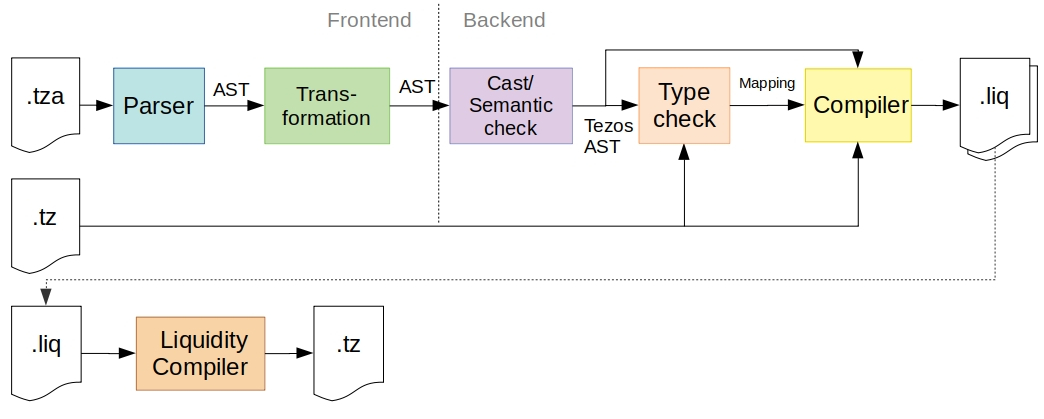
\includegraphics[width=\linewidth]{figures/5-offline_tezos/pipeline_liq}
\caption{Pipeline with IR compilation and an external compiler}
\label{fig:pipeline_liq}
\end{figure}

\paragraph{Comparison to direct compilation}
This approach takes advantage of the usually more sophisticated high-level language compilers; they may provide options for optimizing generated code and are already thoroughly tested. In contrast to large and obscure Michelson programs, the output is more comprehensible and thus easier to test and verify.

The crucial disadvantage of the IR approach is the introduction of an external dependency. The compiler of the respective language has to be extended with the \texttt{random} instruction as well, which requires forking the project. Furthermore, one has to rely on continuous support of new protocol versions in the root project, and integrate the updates into the own code base regularly.

However, a realistic use-case for using Liquidity as an IR is the implementation of the monolithic orchestration scheme. In Liquidity, each entrypoint is declared as a function expecting a parameter and the current storage. During compilation, the contract parameter type and code branching is composed according to the order of functions given in the source file. For instance, the entrypoint declarations in \lstref{lst:liq_eps} are compiled to the contract parameter type \texttt{(or (int \%A) (int \%B))} and two branches in the code body.  
\begin{lstlisting}[numbers=none, label=lst:liq_eps, caption=Entrypoint declarations in Liquidity]
let%entry A (a : int) storage = ...
let%entry B (b : int) storage = ...
\end{lstlisting}
As the Liquidity project provides a decompiler to translate Michelson contracts into Liquidity programs, the compiled assertion functions can simply be appended to the decompiled parent contract. This results in an assembly scheme as depicted in \figref{fig:liq_assembly} and outsources most of the compilation complexity to the Liquidity compiler.

\begin{figure}[t]
\centering
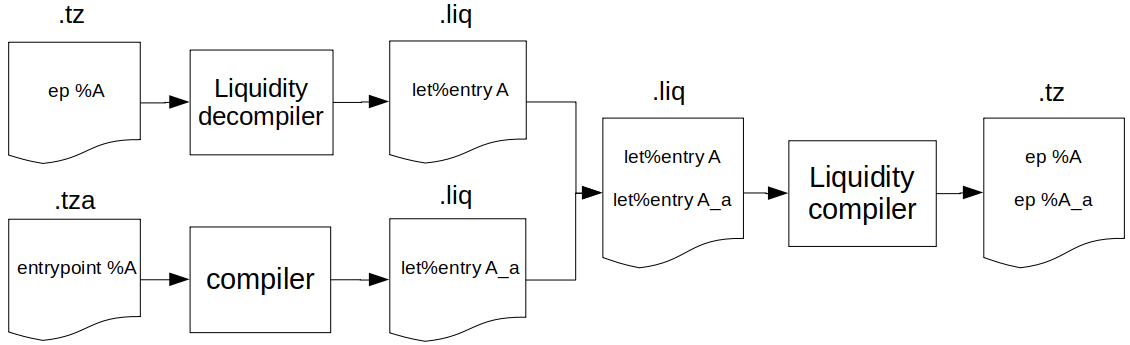
\includegraphics[width=\linewidth]{figures/5-offline_tezos/liquidity_assembly}
\caption{Monolithic assembly using Liquidity as IR}
\label{fig:liq_assembly}
\end{figure}

\section{Cost Analysis and Evaluation}\label{sec:cost_analysis_distributed}
In this section, the costs of checking a formula, with the proposed approach and implementation for distributed assertion checking, are evaluated. \secref{sec:usecase_cost} already determined the cost for a local validation as a benchmark. It stated \eqref{eq:gas_transaction} to calculate the gas consumption of a transaction including internal operations. It identified the gas consumption of deserialization, data parsing and interpretation as growing factors, as they depend on the size of the input parameter.

According to the orchestration scheme, each validator executes $t+2$ operations with the same input parameter $p$. Since they apply lazily, the deserialization cost for the parameter and assertion code only have to be paid once. In addition to the interpretation cost, the reading, parsing and base costs have to be paid for each internal operation. 
\begin{align}\label{eq:gas_validator}
\begin{split}
GasConsumed_{validator}(p) > \quad t * (&base\, gas \\
&+ gasParsing(p) \\
&+ gasRead(C_{assertion}) \\
&+ gasParsing(C_{assertion}) \\
&+ gasInterpretation(C_{assertion})) \\
\end{split}
\end{align}
Based on the resulting inequality in \eqref{eq:gas_validator}, which specifies the costs incurred by each internal operation invoking the assertion contract as a basis of the total gas consumption per validator, it must be concluded that the overall gas consumption of the distributed validation is higher than in the case of a local validation.

The distributed approach was benchmarked by implementing the orchestration scheme for the two minimal dummy contracts \texttt{Foo} and \texttt{Bar} given in \secref{sec:usecase_cost}. Appendix \ref{apx:foobar_distributed} contains the Michelson code for the controller, assertion and parent contracts. In order to preserve comparability between the benchmark of the local and the distributed implementation, the controller contracts were configured with a probability threshold $c = \frac{1}{e}$, s.t. that the necessary number of test runs is equal to the sizes of the search spaces. \figref{fig:cost_distributed} shows the reported gas consumption per validator for different input sizes on the test network Delphinet. Since the effective number of test runs is always a multiple of 32, the cost functions approximate a step function.  

\begin{figure}[t]
\centering
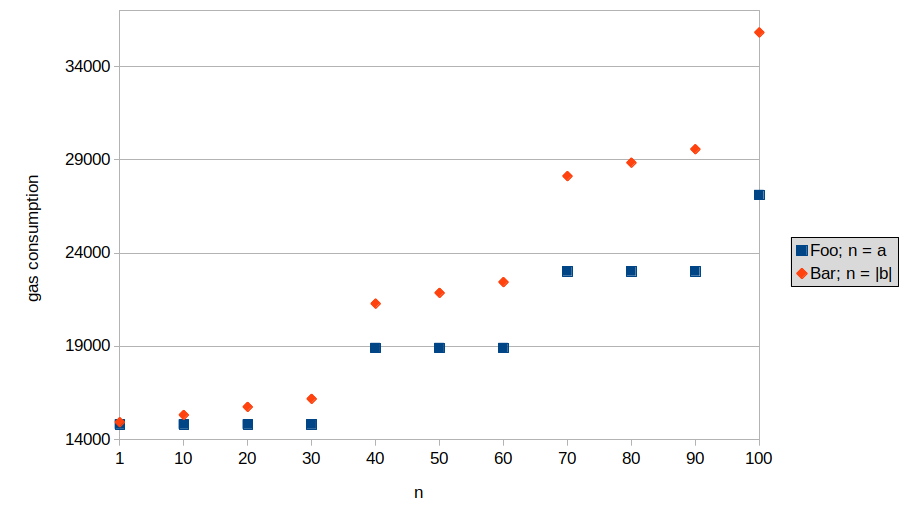
\includegraphics[width=\linewidth]{figures/5-offline_tezos/cost_analysis}
\caption{Gas consumption per validator for different input sizes n}
\label{fig:cost_distributed}
\end{figure}

The results show, that the cost incurred by a single validator, checking a subset of a search space of size $n$, is already considerably higher than a complete validation in a local approach (cf. \figref{sec:usecase_cost}). In the case of the list parameter (contract \texttt{Bar}), the gas consumption even increases exponentially due to the multiplied reading and parsing costs. Moreover, the cost-performance ratio is also worse, as the probability of accepting an invalid parameter with the given configuration is 37\% in the worst case.

In conclusion to these results, the proposed implementation of the distributed scheme has to be evaluated as inefficient and unable to achieve an improvement regarding the scalability of applications on Tezos. However, by reducing the required computation per node to a fraction of the verification, it has the potential to reduce the computational footprint of the transaction within the network. As a prerequisite, it is crucial to lower the costs of the verification. This thesis already mentioned some alternative approaches and implementations, which might achieve this; \secref{sec:alt_random} introduces the possibility to coordinate the validators in a systematic iteration of the search space. Although this does not reduce the cost per test run, it reduces the quantity of necessary test runs to achieve a reliable result. Furthermore, this chapter described several other orchestration schemes, some of which reduce the number of emitted internal operations. As the inter-contract communication accounts for most of the gas consumption in the modular approach, avoiding them is an effective way of reducing the costs. In this regard, a concrete improvement of the proposed architecture could be to merge the controller and assertion code into a single contract. This corresponds, to some extend, to the inverse hybrid architecture as described in \secref{sec:monolithic}. Instead of $t+1$ internal operations, this only requires a single internal operation calling the parent contract (provided that the controller an assertion code are merged into one entrypoint).

\section{Open Questions}
Two remaining aspects of the off-chain design could not be addressed in detail by this thesis. These aspects are outlined briefly in the following sections.

\subsection{Representing Counterexamples}\label{sec:counterexample}
It remains to be specified, how counterexamples are represented within the network. The interaction scheme in \figref{fig:interaction_modular} suggests, that validators publish a counterexample to the network in case of a failed assertion. For this, the validators have to obtain the randomly generated values from within the execution context of the VM. With the \texttt{failwith} instruction, the top element of the stack is exposed, allowing to return an interpretable expression from the execution context. The generated values can thus be returned as a single value, a (nested) pair or a list. To allow other validators to check the assertion with a specific set of values, a modified version of the assertion code must be available on the blockchain. Instead of generating random values, this version should take these values as input parameters. Hence, the validator could create a normal transaction invoking this code with the values returned by the \texttt{failwith} instruction and publish it to the network. The counterexample is then validated like any other transaction on the blockchain. Nodes publishing false counterexamples should be penalized in order to prevent denial of service attacks. After a counterexample has been validated, the respective transaction submitting the invalid off-chain computation should be rejected. Consequently, the transaction and counterexample need to be relatable, e.g. by using an operation hash as an ID. 

To implement this scheme, the compiler has to generate one more contract per assertion. In addition, the assertion contract needs to know about the address of the counterexample contract, and return the address together with the generated values in case of a failure. This requires an adjustment of the storage type of the assertion contract and changes the order of origination to:
\begin{enumerate}
\itemsep-0.5em
\item \texttt{Origination(parent)}, \texttt{Origination(counterexample)}
\item \texttt{Origination(assertion, address counterexample)}
\item \texttt{Origination(controller, [address assertion], address parent)} 
\end{enumerate}

\subsection{Multi-slot Validators}
The proposed implementation assumes that all 32 validators of the current block cycle execute a determined number of test runs. In fact, as mentioned in the section describing Tezos' proof-of-stake mechanism, a validator may have been assigned several endorsement slots per cycle. Since these validators only execute the assertion once, the test runs for the other endorsement slots are neglected. As a result, the error rate of the assertion check is not deterministic and may exceed the configured threshold. This issue should be addressed by the protocol design --- multi-slot validators should execute the assertion check for each of their endorsement slots.